%==============================================================================
%== template for LATEX poster =================================================
%==============================================================================
%
%--A0 beamer slide-------------------------------------------------------------
\documentclass[final]{beamer}
\usepackage{etex}
\usepackage[orientation=portrait,size=a1,
            scale=1.13        % font scale factor
           ]{beamerposter}


\geometry{
  hmargin=1.2cm, % little modification of margins
  vmargin=1.2cm, % little modification of margins
}


% MY PACKAGES
\usepackage[export]{adjustbox}
%\usepackage[demo]{graphicx}
\usepackage{subcaption}

%
\usepackage[utf8]{inputenc}

\linespread{1.12}
%
%==The poster style============================================================
\usetheme{sharelatex}

%==Title, date and authors of the poster=======================================
\title
[Probabilistic Graphical Models Poster Session, Wed 4 Jan 2017] % Conference
{ % Poster title
Alignment models for statistical translation
}

\author{ % Authors
Thomas Debarre, Matthieu Kirchmeyer, Sylvain Truong, Nicolas Zhang
}
%\institute{}
\institute
%[Very Large University] % General University
{\mbox{}
%\inst{1} Very Large University, Neverland\\[0.3ex]
%\inst{2} Other University, Neverland\\[0.3ex]
%\inst{3} Yet Another University, Neverland
}
\date{\today}



\begin{document}
\begin{frame}[t]
%==============================================================================
\begin{multicols}{3}
%==============================================================================
%==The poster content==========================================================
%==============================================================================

\section{Introduction}

This project explores three methods to solve the problem of word alignments for a bilingual corpus from the conventional mixtures models (\textbf{IBM1}, \textbf{IBM2}) to a first-order Hidden Markov model (\textbf{HMM}) developped in \cite{vogel}. 

%The goal is to translate a text given in a language (French in all that follows) to another language (English) taking into account one-to-many alignments or null words; the quality of the translation relies on the quality of the word alignments.
The goal is to understand the underlying lingustic bonds that exist between two languages (French and English in all that follows). These bonds are here addressed with the problem of word alignments in translated French-English sentence pairs.

We evaluated our algorithms on a small bilingual French-English dataset $\mathcal{D} = \{ (\textbf{f}^{(1)},\textbf{e}^{(1)}), \dots , (\textbf{f}^{(N)},\textbf{e}^{(N)})\}$ which consists of $N = 22$ French sentences composed of 4 to 10 words with their translated English equivalents. 

\section{Statistical translation models}

\subsection{IBM models}
The IBM alignment models for statistical machine translation were introduced by IBM more than 20 years ago \cite{brown}. In this project, we implemented the 2 most basic IBM models, IBM1 and IBM2. Both these models are based on the decomposition of the joint probability of a French sentence $\textbf{f}$ of length $I$ and its alignment $\textbf{a}$ conditioned on the English sentence $\textbf{e}$ of length $J$:
\begin{equation*}
p(\textbf{f}, \textbf{a} \vert \textbf{e}) = p(I \vert J) \prod_{i=1}^I p(a_i \vert i, J, I) \cdot p(f_i \vert e_{a_i})
\end{equation*}
The alignment vector $\textbf{a} = (a_1, \hdots, a_I)$ maps a French word $f_i$ in $\textbf{f}$ to an English word $e_{a_i}$ in $\textbf{e}$. We have $a_i \in [0, J]$, where $a_i = 0$ is the \textit{null alignment}.

The goal is to learn the probabilistic model of a French sentence given an English sentence $p_\Theta (\textbf{f} \vert \textbf{e})$, where $\Theta = \lbrace  p(f \vert e)\rbrace$ is the set of parameters of the model, $f$ and $e$ being the French and English words appearing in the training dataset.

To learn this model, the \textbf{EM algorithm} is used, where the alignment is the latent variable. The \textbf{Expectation step} consists in calculating $\mathbb{E}(count \langle f, e \rangle)$, the expected number of times the French word $f$ is aligned with the English word $e$. Next, the \textbf{Maximization step} updates the parameters of the model using $\hat{p}(f \vert e) \propto \mathbb{E}(count \langle f,e \rangle)$.

Once the model has been trained, it can be decoded by calculating the most likely alignment $\hat{\mathbf{a}} = \underset{\mathbf{a}}{\mathrm{argmax}} \ p(\mathbf{a} \vert \mathbf{f}, \mathbf{e})$ for a pair of translated sentences $(\textbf{f}, \textbf{e})$.
\medskip
\begin{center}
\structure{IBM1} 
\end{center}
\medskip

The IBM1 model assumes that a word of a French sentence has an equal probability of being aligned with any word of the corresponding English sentence (including the null word), i.e. 
\begin{equation*}
p(a_i = j \vert i, J, I) = p(a_i = j \vert J) = \frac{1}{J + 1}
\end{equation*}
Therefore, IBM1 exclusively relies on lexical translation; the ordering of the words in sentence is unaccounted for. The decoding of the model is straightforward: the most likely alignment for a pair of translated sentences $(\textbf{f}, \textbf{e})$ is given by $\hat{a_i} =\underset{j}{\mathrm{argmax}} \ p(f_{i} \vert e_{j})$

\medskip
\begin{center}
\structure{IBM2} 
\end{center}
\medskip

The IBM2 model assumes that alignments of words that are around the same relative place in their respective sentences are more likely, i.e. 
\begin{equation*}
p(a_i = j \vert i, J, I) \propto b( \vert \frac{i}{I} - \frac{j}{J} \vert) \qquad j \neq 0
\end{equation*}
where $b: \mathbb{R}^{+} \to [0, 1]$ is a decreasing function. The probability of the null alignment ($j=0$) is a fixed parameter $p_0$. We chose $b: t \mapsto \exp (- \lambda t)$, where $\lambda$ is a tuning parameter (\cite{dyer}).

The decoding of the model is still quite simple: the most likely alignment for a pair of translated sentences $(\textbf{f}, \textbf{e})$ is given by $\hat{a_i} =\underset{j}{\mathrm{argmax}} \ p(a_i = j \vert i, J, I) p(f_{i} \vert e_{j})$.

IBM2 is still rather simplifying since it only takes into account the absolute position of words in a sentence. This is why HMM-based alignment models were introduced to account for the relative position of words.

\subsection{HMM-based alignment models}

The HMM-based alignment models were introduced by \textit{Vogel and al.}(1996) and aim at modeling the joint probability of a French sentence $\textbf{f}$, of length $J$ and an alignment $\textbf{a}\in \{1,\dots,I\}^J$, given a English sentence $\textbf{e}$ of length $I$.
Without, loss of generality, this probability can be expressed as (chain-rule and independance of $\textbf{f}$ and $\textbf{a}$):
\begin{align*}
Pr(\textbf{f},\textbf{a}|\textbf{e}) &= Pr(f_0,a_0|\textbf{e}) \prod_{j=1}^J Pr(f_j,a_j|f_{1}^{j-1},a_{1}^{j-1},\textbf{e})\\
&= Pr(f_0|\textbf{e}) \cdot Pr(a_0|\textbf{e})\\
&\cdot \prod_{j=1}^J Pr(f_j|f_{1}^{j-1},a_{1}^{j-1},\textbf{e}) Pr(a_j|f_{1}^{j-1},a_{1}^{j-1},\textbf{e})
\end{align*}

The HMM model reduces the generality of the previous formula by assuming first-order dependance of alignments and translation probability of French word at position $j$ to be only dependent on the English word at position $a_j$, thus yielding the HMM model:

\begin{align*}
Pr(\textbf{f},\textbf{a}|\textbf{e}) &= p(f_0|e_{a_0}) p(a_0)\\
&\cdot \prod_{j=1}^J p(f_j|e_{a_{j}}) \cdot p(a_j|a_{j-1},I)
\end{align*}

\vskip1ex
\begin{figure}
\centering
%\includegraphics[width=0.99\columnwidth]{logo.png}
\adjincludegraphics[width=0.99\columnwidth,trim={{0.03\width} {0.6\height} {0.02\width} 0},clip]{figures/hmm.pdf}
\caption{The HMM-based alignment model}
\label{fig:hmm_model}
\end{figure}
\vskip2ex

Figure~\ref{fig:hmm_model} presents the graphical model associated with HMM-based alignment models. What can be noticed is that, in this context, each sentence pair represents a Hidden Markov Model which parameters are shared with all other sentences of the corpus.
The \textbf{parameters for the HMM model} are
\begin{align*}
\Theta &= \lbrace\\
& p(i) &\mbox{   the initial alignment probabilities ($p(a_0=i)$)}\\ 
& p(i|i',I) &\mbox{   the transition matrix ($p(a_{j+1}=i|a_{j}=i')$)}\\
& p(f|e) &\mbox{   the emission (translation) probabilities}\rbrace
\end{align*}

A further assumption from \textit{Vogel and al.} is that alignment transition probabilities \textbf{only depend on relative positions}: $p(i|i',I) = p(i'-i|I)$

Just as for the IBM models, the observations are the sequences of French words in French sentences, while the alignments (and thus the corresponding English words) act as hidden variables. A way to solve this problem is, again, to use an \textbf{EM principle}.
The \textbf{Expectation step} consists in computing alignment unary and binary probabilities in \textbf{each sentence pair} $(\textbf{f},\textbf{e})$. 

\begin{align*}
\gamma_i(j) &= p(a_j=i|\textbf{f})\\
\xi_{k,l}(j) &= p(a_j=k,a_{j+1}=l|\textbf{f})
\end{align*}
\vskip1ex
This can be performed using the \textbf{Forward-Backward} algorithm.
The \textbf{Maximisation step} consists in re-estimating the model's parameters according to the previously computed probabilities. This step broadly consists in aggregating the $\gamma$ and $\xi$ probabilities for all $(\textbf{f},\textbf{e})$ sentence pairs (\cite{anahita}).

The \textbf{Viterbi} decoding algorithm is then used to retrieve the most likely alignments in the corpus, according to the computed transition and emission probabilities.

\section{Results and discussions}

%\subsection{Proposed evaluation method}
%
%\subsection{Example results}

\begin{figure}
\centering
%\includegraphics[width=0.99\columnwidth]{logo.png}
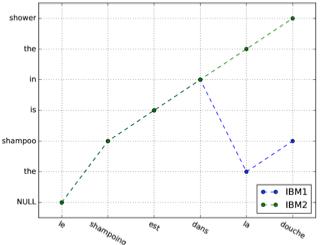
\includegraphics[width=0.75\columnwidth, height=.7\columnwidth]{figures/ibm1_2.png}
\caption{Comparison of the IBM models 1 and 2 example }
\label{fig:ibm}
\end{figure}
\begin{figure}
\centering
\begin{subfigure}{.80\columnwidth}
  \centering
  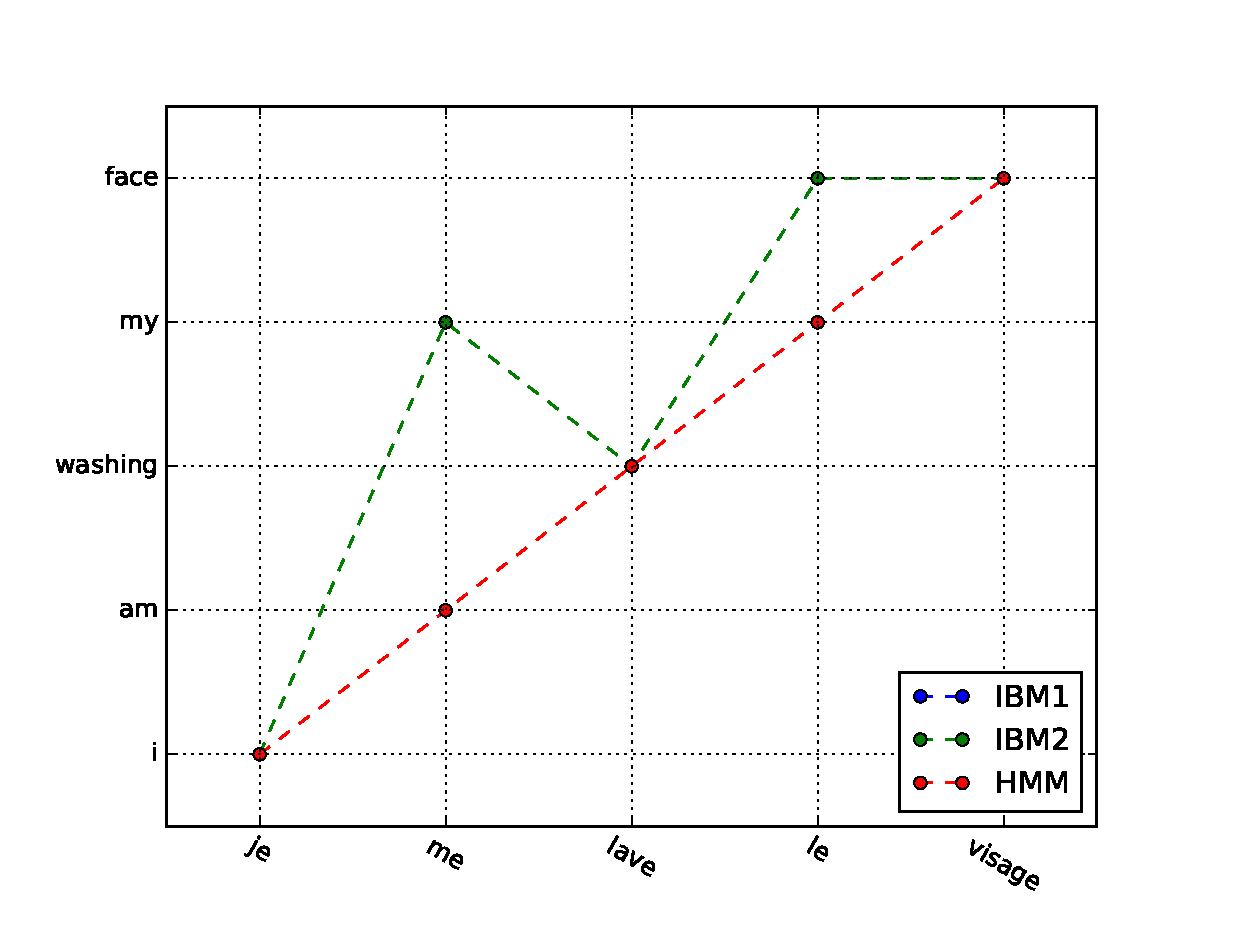
\includegraphics[width=.99\linewidth]{figures/figures_final/sentence3.eps}
\end{subfigure}%

\begin{subfigure}{.80\columnwidth}
  \centering
  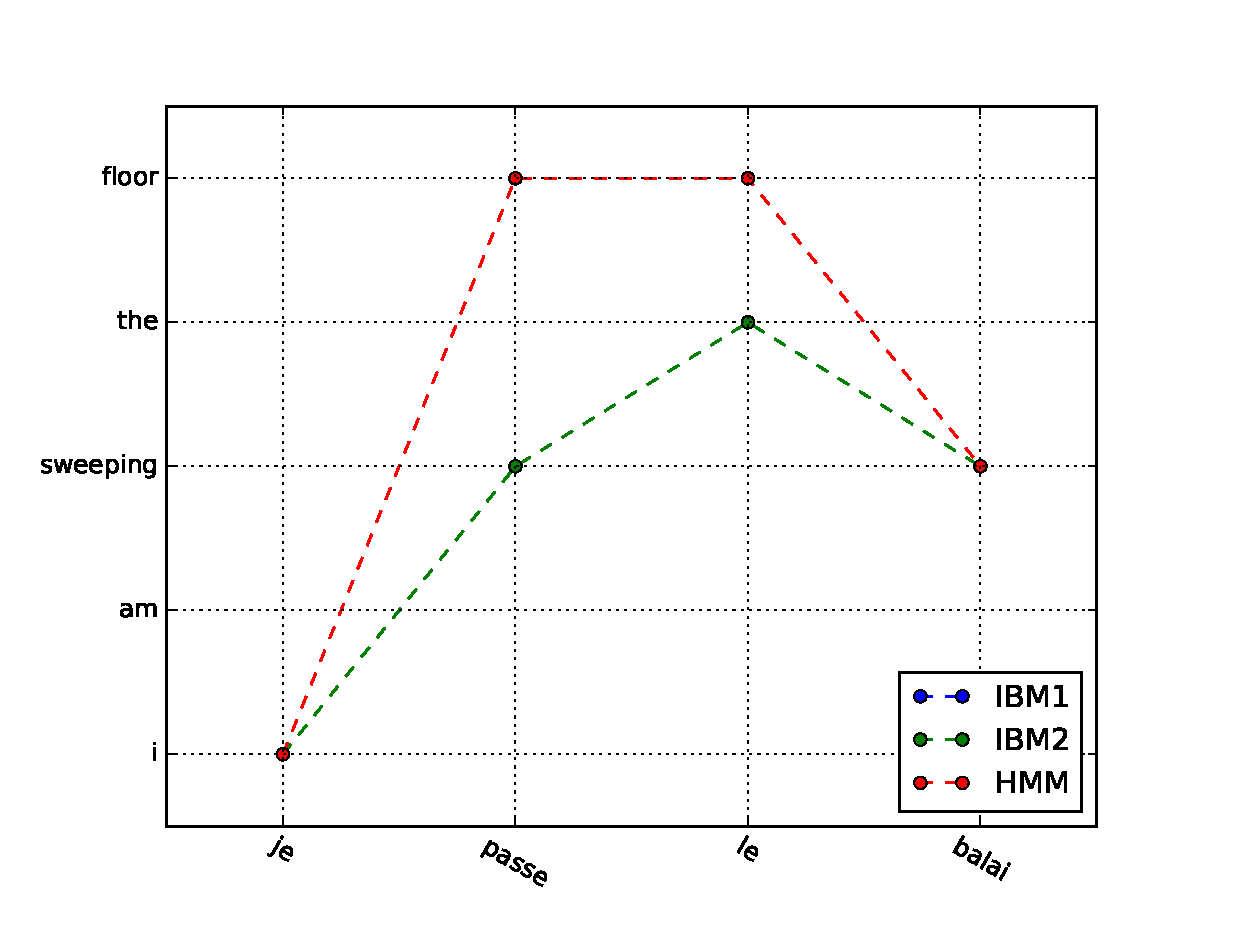
\includegraphics[width=.99\linewidth]{figures/figures_final/sentence11.eps}
\end{subfigure}%
\caption{Comparison of the IBM models and HMM model }
\label{fig:hmm}
\end{figure}

%\vskip1ex
%\begin{figure}
%\centering
%%\includegraphics[width=0.99\columnwidth]{logo.png}
%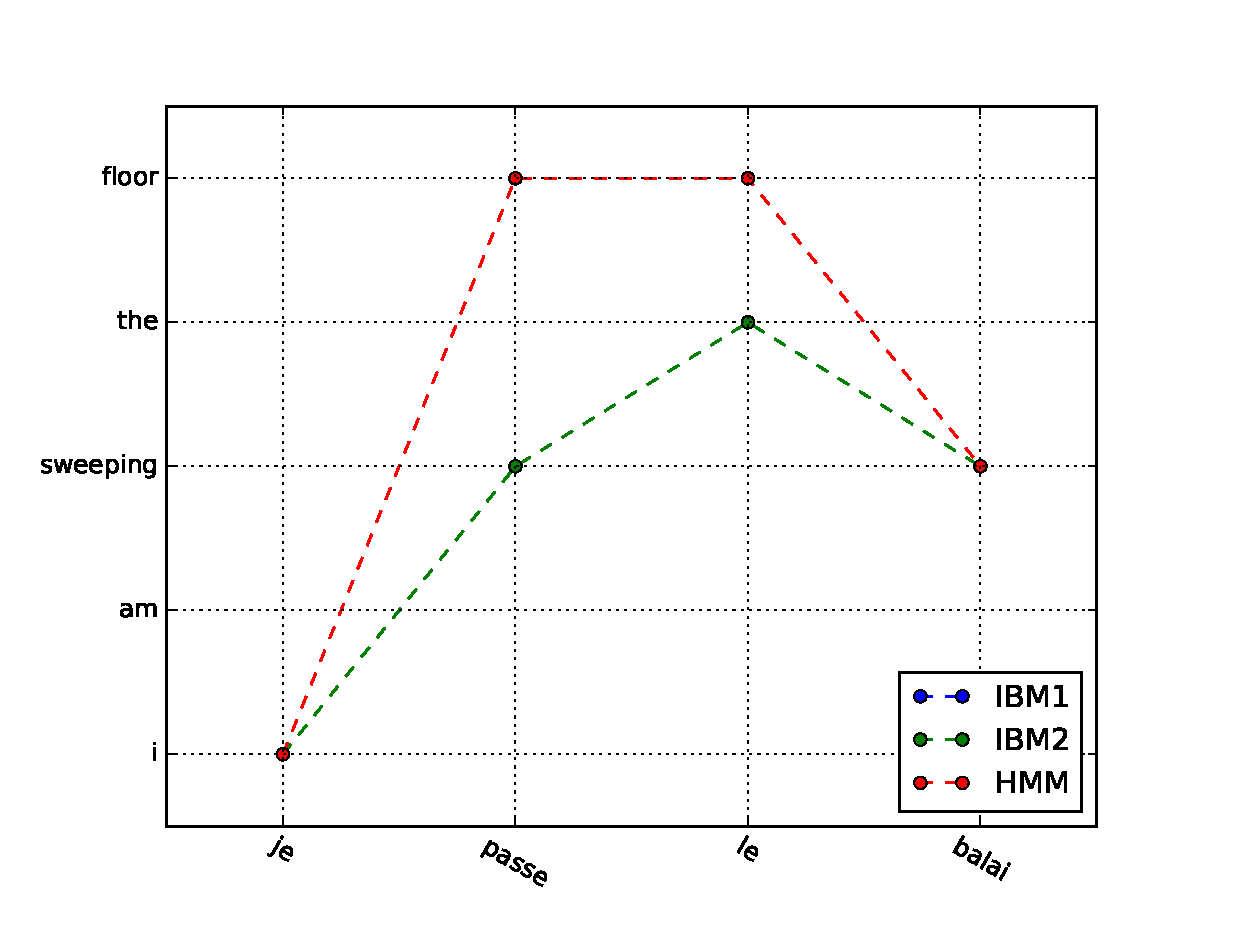
\includegraphics[width=0.99\columnwidth, height=.7\columnwidth]{figures/figures_final/sentence11.eps}
%\caption{Comparison of the IBM models 1 and 2 example }
%\label{fig:ibm}
%\end{figure}
%\vskip1ex
%\begin{figure}
%\centering
%%\includegraphics[width=0.99\columnwidth]{logo.png}
%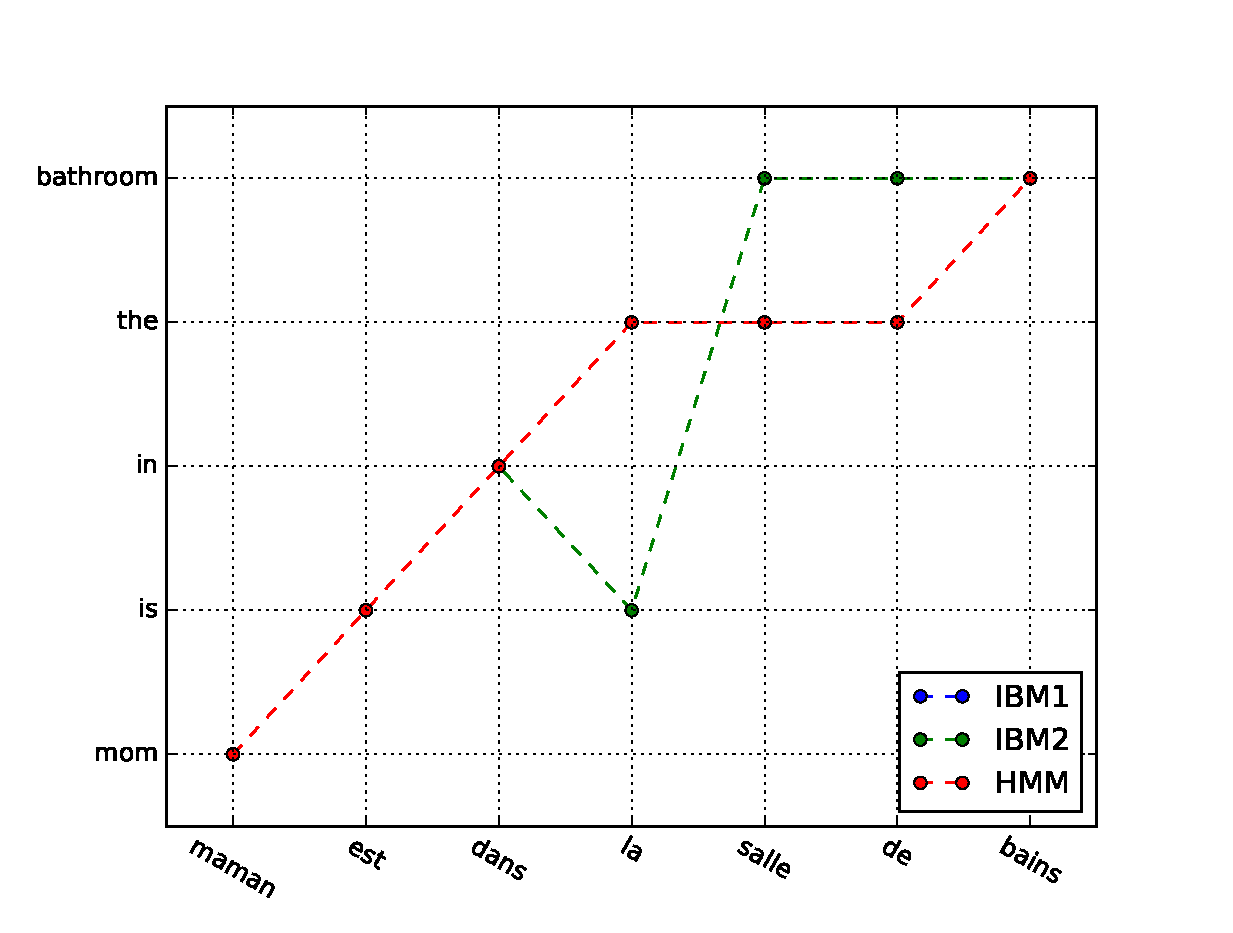
\includegraphics[width=0.99\columnwidth, height=.7\columnwidth]{figures/figures_final/sentence8.eps}
%\caption{Comparison of the IBM models 1 and 2 example }
%\label{fig:ibm}
%\end{figure}
%\vskip1ex
%\begin{figure}
%\centering
%%\includegraphics[width=0.99\columnwidth]{logo.png}
%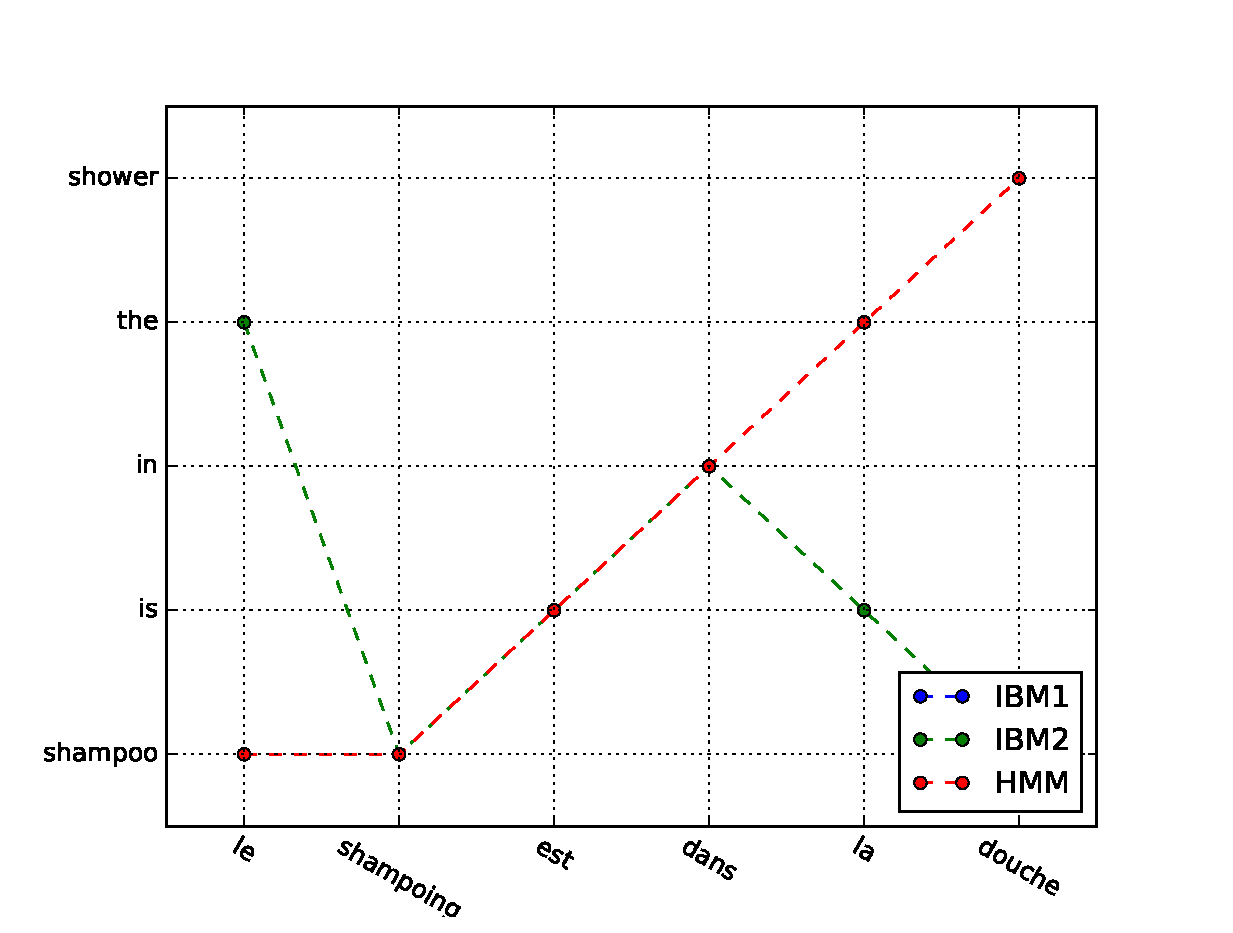
\includegraphics[width=0.99\columnwidth, height=.7\columnwidth]{figures/figures_final/sentence5.eps}
%\caption{Comparison of the IBM models 1 and 2 example }
%\label{fig:ibm}
%\end{figure}
%\vskip2ex

Figure~\ref{fig:ibm} shows an example of the decoding results with IBM models 1 and 2 for a same sentence pair. It shows the improvement of IBM2 over IBM1: the English word "the" appears twice in the English sentence, so the IBM1 does not make any distinction between them. However, IBM2 takes the position of words into account, so since the French word "la" is towards the end of the sentence, it is aligned with the second "the".

Figure~\ref{fig:hmm} shows examples of HMM-based runs. The overall straighter alignments can be interpreted as an influence of taking into account relative positions of alignments. In practice, HMM-based trainings require homogeneous number of words in the English corpus (conditioning on $I$ in the transition matrix), and are harder, but also longer, to train. 

\section{Conclusion}

We compared in this project an HMM-based approach for modelling word alignments with mixture alignment models (IBM1/2). The translation probabilities produced by the HMM model are comparable to the IBM1/2 models with smoother position alignments as it makes alignment probabilities dependent on the alignement position of the previous word. Futher work could involve extending the HMM alignment model by addressing empty word problem or fertility which were not taken into account in the developped model.

%==============================================================================
%==End of content==============================================================
%==============================================================================

%--References------------------------------------------------------------------

\subsection{References}

\begin{thebibliography}{99}

\bibitem{vogel} S. Vogel, H. Ney, and C. Tillmann, HMM-based word alignment in statistical translation, 1996

\bibitem{brown} P. Brown et al., The Mathematics of Machine Translation: Parameter Estimation, 1993

\bibitem{dyer} C. Dyer et al., A Simple, Fast, and Effective Reparameterization of IBM Model 2, 2013

\bibitem{anahita} Bigvand, A. M., Word Alignment for Statistical Machine Translation Using Hidden Markov Models, 2015

\end{thebibliography}
%--End of references-----------------------------------------------------------

\end{multicols}

%==============================================================================
\end{frame}
\end{document}